\documentclass[12pt,dvipdfmx,mathserif,uplatex,aspectratio=32]{beamer}
\usetheme{Singapore}
\AtBeginShipoutFirst{\special{pdf:tounicode EUC-UCS2}}
\usepackage{euler}
\usepackage{multicol}
\usepackage{subfigure}
\usepackage{graphicx}
\renewcommand{\kanjifamilydefault}{\gtdefault}
\setbeamerfont{title}{size=\LARGE}


\title{パケット分類について}
\subtitle{2015年度 前期輪講 \\ "Survey and Taxonomy of Packet Classification Techniques" \\ Abstract and Introduction}
\author{原田崇司}
\date[]{2015年4月21日}
\institute[所属]{神奈川大学大学院 理学研究科 情報科学専攻 田中研究室}
% [..]に省略名が書ける

\begin{document}

\frame{\maketitle}

\section*{内容}


\begin{frame}{目次}
  \tableofcontents
\end{frame}



\section{フィルタリング}


\begin{frame}{フィルタリングルール}
% daggerについて説明
% FlowID(Permit, DenyなどのAction)について説明
% nonexclusive filter, exclusive filter
% nonexclusive filter, parameter r について質問

\begin{table}
 \begin{tabular}{|l|l|l|l||r|c|} \hline
 \multicolumn{4}{|c||}{Filter} & \multicolumn{2}{|c|}{Action} \\ \hline
 SA & DA & Prot & DP & FlowID & PT  \\ \hline
 $11010010$ & $*$        & TCP  & [$3:15$] & $0$  & $3$  \\
 $10011100$ & $*$        & $*$  & [$1:1$]  & $1$  & $5$ \\
 $101101*$  & $001110*$  & $*$  & [$0:15$] & $2$  & $8^{\dagger}$ \\
 $10011100$ & $01101010$ & UDP  & [$5:5$]  & $3$  & $2$ \\
 $*$        & $*$        & ICMP & [$0:15$] & $4$  & $9^{\dagger}$ \\
 \multicolumn{1}{|c}{\vdots} & \multicolumn{1}{|c}{\vdots} & \multicolumn{1}{|c}{\vdots} & \multicolumn{1}{|c||}{\vdots} & \multicolumn{1}{|c}{\vdots} & \multicolumn{1}{|c|}{\vdots} \\
 $01110010$ & $*$        & TCP  & [$3:15$] & $12$ & $4^{\dagger}$\\
 $10011100$ & $01101010$ & TCP  & [$0:1$]  & $13$ & $3$ \\
 $01110010$ & $*$        & $*$  & [$3:3$]  & $14$ & $3$ \\
 $100111*$  & $011010*$  & UDP  & [$1:1$]  & $15$ & $4$ \\ \hline
 \end{tabular}
 %\caption{Example Rulelist}
\end{table}

\end{frame}

\begin{frame}{フィルタリングの例}

{\centering
SA$=10011100$,DA$=01101010$,Prot$=$UDP, DP$=1$

}
\begin{table}
 %\caption{Example Rulelist}
{\centering

 {\small
 \begin{tabular}{|l|l|l|l||r|c|c} \cline{1-6}
 \multicolumn{4}{|c||}{Filter} & \multicolumn{2}{|c|}{Action} & \\ \cline{1-6}
 SA & DA & Prot & DP & FlowID & PT  & \\ \cline{1-6}
 $11010010$ & $*$        & TCP  & [$3:15$] & $0$  & $3$ & \\
 \color{red}$10011100$ & \color{red}$*$        & \color{red}$*$  & \color{red}[$1:1$]  & \color{red}$1$  & \color{red}$5$ & \\
 $101101*$  & $001110*$  & $*$  & [$0:15$] & $2$  & $8^{\dagger}$ & \\
 $10011100$ & $01101010$ & UDP  & [$5:5$]  & $3$  & $2$ & \\
 $*$        & $*$        & ICMP & [$0:15$] & $4$  & $9^{\dagger}$ & \\
 \multicolumn{1}{|c}{\vdots} & \multicolumn{1}{|c}{\vdots} & \multicolumn{1}{|c}{\vdots} & \multicolumn{1}{|c||}{\vdots} & \multicolumn{1}{|c}{\vdots} & \multicolumn{1}{|c|}{\vdots} & \\
 $01110010$ & $*$        & TCP  & [$3:15$] & $12$ & $4^{\dagger}$ & \\
 $10011100$ & $01101010$ & TCP  & [$0:1$]  & $13$ & $3$ & \\
 $01110010$ & $*$        & $*$  & [$3:3$]  & $14$ & $3$ & \\
\color{red}$100111*$  & \color{red}$011010*$  & \color{red}UDP  & \color{red}[$1:1$]  & \color{red}$15$ & \color{red}$4$ & \color{red} \scalebox{0.4}{\includegraphics{redleftarrow.eps}} \\ \cline{1-6}
 \end{tabular}

 }

}
\end{table}

\end{frame}


\begin{frame}{NonExclusive Filter}

{\centering
\input{rbtrie.tps}

}

\end{frame}

\begin{frame}{NonExclusive Filter}

{\centering
\scalebox{0.75}{\input{predtree.tps}}

}

\vspace{5mm}

{\centering

Run-Based Trieの決定木は,NonExclusive Filterに対応しない
}

\end{frame}

\begin{frame}{テーブル探索の複雑さ}

効率的なテーブル探索は難しい問題 \\
\vspace{3mm}
\scalebox{0.5}{
\includegraphics{rightarrow.eps}}
ネットワークにおける,パフォーマンスボトルネック

\vspace{5mm}
{\centering
\includegraphics{downarrow.eps}

}

\vspace{5mm}

{\centering
遅延を減らすパケット分類技術が必要


}

\end{frame}


\begin{frame}{パケットフィルタリング技術}

\begin{itemize}
 \item アルゴリズムによる方法 \vspace{2mm}
   \begin{itemize}
     \item[-] 決定木などのデータ構造を用いる方法 \vspace{2mm}
       \begin{itemize}
         \item[*] HiCuts \vspace{1mm}
         \item[*] Run-Based Trie \vspace{1mm}
         \item[*] 階層型トライ \vspace{1mm}
       \end{itemize} \vspace{2mm}
     \item[-] ルールリスト並び替えによる遅延を減らす方法 \vspace{2mm}
       \begin{itemize}
         \item[*] Sub-Graph Merging \vspace{1mm}
         \item[*] 昆金法 \vspace{1mm}
         \item[*] 竹山法 \vspace{1mm}
       \end{itemize} \vspace{2mm}
   \end{itemize}
 \item アーキテクチャによる方法
   \begin{itemize}
     \item Ternary Content Addressable Memory
   \end{itemize}
\end{itemize}

\end{frame}


\section{フィルタリングにおける制約,状況}


\begin{frame}{通信速度}

現在の通信速度 \\ \vspace{2mm}
\begin{itemize}
 \item UTP ケーブル:$1Gbs$(Cat5,6),$10Gbs$(Cat6e.7)
       %Unshielded Twisted Pair
       %Shielded Twisted Pair ケーブル
       %カテゴリは,伝送距離,最大周波数に関係する区分
 \item 光ケーブル :$1Pbs$ (NTT,北大,その他)
       %P = $10^{15}$
\end{itemize}

\vspace{3mm}

TCPでは,通信路を確保し,確認応答を行う.\\
(データ受信受信側が,受信した証に送信元へサイズが$40$バイトのパケットを送る) \\
%$10Gb/s$のリンクは,一秒間に$31M$のパケットを処理する能力をルータに求める

{\centering
\includegraphics{downarrow.eps}

}

例.$10Gb$の通信速度をサポートするルータは,ポートごとに($10^{9}/(40\times8) =$) $3.125 \times 10^{7}pps$の処理能力を要求される.
%pps(Packet Per Second)
%リンクの速度とTCPのACKを基準にしているため

\end{frame}


\begin{frame}{フィルタリングアルゴリズムの性能}

ほとんどのアルゴリズムは,平均的には十分なものである.\\
\vspace{10mm}

しかし,病的な場合の探索能力を考えなければならない\\
(一番都合の悪いフィルタ,パケットがくる場合)

\vspace{10mm}
\begin{itemize}
 \item ネットワーク :最悪の処理能力を保証する
 \item インターネット:処理能力を保証しない,\\ \hspace{32.3mm}ベストエフォートサービスを提供
\end{itemize}

\end{frame}


\begin{frame}{ルータの性能}

入出力ポートが同じである充分に長いパケットを考える.\\
\vspace{3mm}
\scalebox{0.5}{
\includegraphics{rightarrow.eps}} \hspace{1mm} バッファが溢れてしまう.\\

\vspace{5mm}
{\centering
\includegraphics{downarrow.eps} \\

}
\vspace{5mm}

{\centering
ルータのスイッチング技術は,最悪の状況には対応できない.

}

\end{frame}


\begin{frame}{フィルタリングルール数}

インターネットの爆発的な成長 \\ \vspace{3mm} \scalebox{0.5}{
\includegraphics{rightarrow.eps}} \hspace{1mm} ルール数の増加(エントリ数$2 \sim 3k \rightarrow 10k$)

\vspace{5mm}

{\centering
\includegraphics{downarrow.eps} \\

}

\vspace{5mm}

{\centering
拡張可能性,$10~100k$エントリのルールリストを考慮

}

\end{frame}

%% 1秒間に1兆ビットの転送ができるレベルになると
%% エネルギー消費量も重要な観点になる



\section{問題の回避}

\begin{frame}{IP lookupsとIPパケット分類の回避}
転送を加速させるために,IPヘッダの情報を使わない.\\
%宛先情報を使用しない

\vspace{10mm}

ヘッダ情報を使わない?アルゴリズム
\begin{itemize}
 \item MPLS
 \item Tag-Switching %パケット情報を圧縮
 \item ATM仮想回線(ATM Virtual Circuit)
\end{itemize}

\end{frame}


\begin{frame}{Multi Protocol Label Switching}

{\centering
\scalebox{0.5}{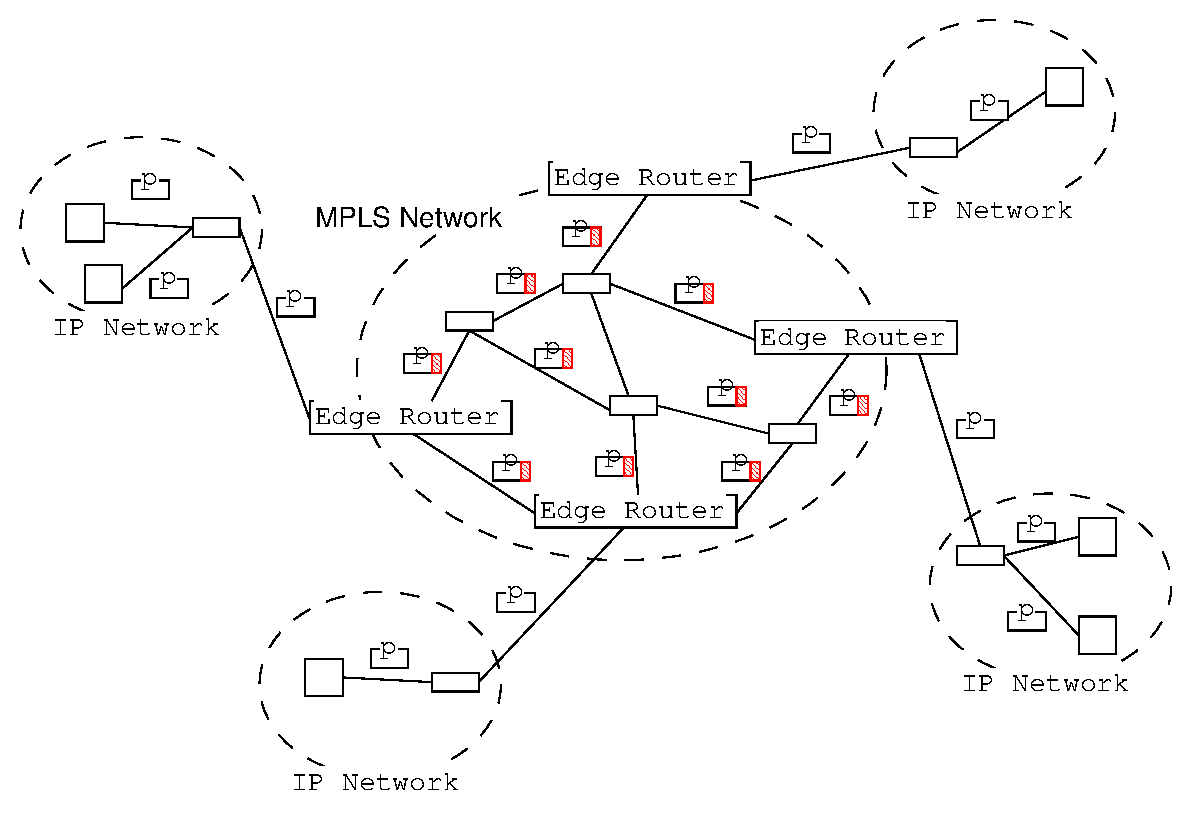
\includegraphics{mpls.eps}}

}
\end{frame}

\begin{frame}{IP情報回避の問題}
確かに,自律システム内では使用していない \\
\vspace{3mm}
しかし,境界上のルータは,パケットをラベル付けする \\ \vspace{1mm}(分類する)必要がある \\

\vspace{5mm}
{\centering
\includegraphics{downarrow.eps} \\

}
\vspace{5mm}

{\centering
{\LARGE \color{red}パケット分類技術は必要且つ重要}

}

\end{frame}


\end{document}
